\documentclass[a4paper,10pt,reqno,oneside]{amsart}
%\usepackage[small]{caption}
%\usepackage[usenames,dvipsnames]{color}
%\usepackage[colorlinks=TRUE,linkcolor=Black,urlcolor=Black,citecolor=Black,pagebackref=TRUE,]{hyperref} %Have to change href email.
\usepackage{amsfonts,fancyhdr,graphicx,lastpage,rotating,multirow,fixltx2e, stfloats,txfonts,palatino,url,xcolor,multicol,hanging, setspace,lscape, paralist, changepage,program,subcaption,array,verbatim,setspace}
\usepackage[pagewise,displaymath, mathlines]{lineno}
\usepackage{epstopdf}



\usepackage[nolists, nomarkers]{endfloat}
\linenumbers
\doublespacing

\usepackage[sort&compress,comma]{natbib}
%\newcolumntype{H}{@{}>{\lrbox0}l<{\endlrbox}}


\renewcommand{\theequation}{eqn \arabic{equation}}





\begin{document}


\title{A generalisation of REM models for camera traps or acoustic sensors}
\maketitle

\noindent {\bf Running title: REM models for camera traps or acoustic sensors}

\noindent {\bf Word count:}

\noindent {\bf Authors:\\}
Tim C.D. Lucas\textsuperscript{1,2,3*}, Elizabeth Moorcroft\textsuperscript{1,4,5}, Kate E. Jones\textsuperscript{2,5}, Marcus J. Rowcliffe\textsuperscript{5}, Robin Freeman\textsuperscript{5}\\


\noindent {\bf Addresses:\\}
1 CoMPLEX, University College London, Physics Building, Gower Street, London, WC1E 6BT, UK\\ 
2 Department of Genetics, Environment and Evolution, UCL, Gower Street, London, WC1E 6BT, UK\\ 
3 Department of Statistical Science, University College London, Gower Street, London, WC1E 6BT, UK\\ 
4 Department of Computer Science, University College London, Gower Street, London, WC1E 6BT, UK\\ 
5 Institute of Zoology, Zoological Society of London, Regents Park, London, NW1 4RY, UK


\noindent {\bf Corresponding author:\\}
Tim C.D. Lucas,\\
CoMPLEX,\\
University College London,\\
Gower Street,\\
London,\\
WC1E 6BT, \\
UK\\
timcdlucas@gmail.com\\


\clearpage


%max word count 250 words. Currently too long.

\section{Abstract}
Point 1: Camera traps and acoustic detectors are becoming common in ecology but the methods needed to estimate population abundance and density with these technologies, specifically when individuals are not identifiable, are not established. Both camera traps and acoustics detectors are becoming cheaper and more practical for broad scale ecological studies. However, their usefulness is currently limited by a lack of methods to estimate population densities and abundance. Current methods often require individual identification or an estimate of the distance from the animal to the sensor

Point 2: We have generalised the 'ideal gas' model to account for camera traps and acoustic detectors that cannot detect animals within a full 360 degree arc and to account for animals whose acoustic calls are directional. We model both animals and sensors as geometric shapes and drive equations for the expected number of encounters per unit time between the animal population and the sensor. The models are tested using spatially explicit simulations. 

Point 3: The resultant models are suitable for any combination of sensor width and call directionality. We find that the models give an unbiased estimate of density. The precision of the estimate increases with effective survey effort. The estimate remains remains unbiased under the range of assumptions about animal movement. 

Point 4: These models provide an effective, and currently the only, method to estimate animal abundance when animals are individually unidentifiable and the distance between sensor and animal is unknown. This allows estimates of abundance for a range of taxa that have been currently very hard to study using teleprinter cheap technologies that can be spread over wide areas and left to run autonomously. Furthermore, the ability to estimate absolute abundance rather than relative abundance or indices is important in a range of fields such as disease dynamics, conservationgenetics and ecosystem services. 

\subsection{Keywords}
Gas model, acoustic detection, abundance estimate, random encounter model, bat detector, camera trap

\section{Introduction}

\begin{itemize}
\item Monitoring the size of populations is necessary for maintaining biodiversity.
\item Monitoring can be done in different ways, by a direct count or through taking samples. \citep{pollock2002large}
\item Methods for collecting samples can vary from human surveys to sensor records, such as the results from cameras or sound recorders placed throughout an environment. 
\item Sensors are growing in popularity, as they are efficient, relativity cheap and non-invasive. \citep{gese2001monitoring}
\item Samples collected from sensors can then be used in methods like REM or Capture-Recapture in order to estimate density of the population.
\item Current methods are not suitable for all species, so some species have no, or unreliable, population information. 
\item These species are often difficult to capture on camera, but are easier to detect using an acoustic sensor \citep{rogers2013density}, such as bats \citep{ofarrel1999comparison}, whales \citep{mcdonald1999passive}, and potentially for species such as monkeys. 
\item But these data collection methods are incompatible with REM, because the width of the sensor can be greater than 90, and because the animal may give off a directional signal 
\item We are going to extend REM methods so that it can be used with acoustic data as well as data collected via camera traps
\end{itemize}

\subsection{Hypotheses}

\begin{itemize}
\item The analytical model can accurately predict density when the assumptions of a homogeneous environment and straight-line animal movement are met.
\item The accuracy of the model is not affected by changes in the movement model, however the precision of the analytical models are affected
\item The precisions of the analytical models are also affected by sampling effort, radius of detection, call angle and detection angle, animal speed and density.
\end{itemize}

\subsection{Aims}

\begin{itemize}
\item  In this study we created a general model, as an extension to the REM, to estimate absolute abundance from count data from acoustic or visual sensors. Where the angle of detection of the sensor can vary from 0 to 360°, and the signal given off from the animal can be between 0 and 360°.
\item  We tested the model using simulations in order to:
\begin{itemize}
\item Access the validity, i.e. that the bias is equal to 0
\item  To be able to give suggestions for best practice
\end{itemize}
\end{itemize}


\section{Methods}

\subsection{Analytical Model}

In this section we outline the general process for deriving the models. However, as the full derivation is long, it is included in the supplementary material.

The model presented by \citep{rowcliffe2008estimating} is derived assuming a sensor with a viewing angle less than $\pi/2$ radians and so the sensor is modeled as a circular segment with a central angle between 0 and  $\pi/2$ named  $\theta$.

Furthermore, as they modeled a camera trap, an animal can be detected from any direction. We however want to relax this assumption to allow for acoustically detected animals. We therefore model the animal as having an associated call angle $\alpha$.

In general we are aiming to derive models for any sensor angle, $ \theta$, between 0 and $2\pi$ and any call angle, $ \alpha$, between 0 and $2\pi$. We can easily derive the gas model which is the case where $ \alpha =  2\pi$ and $ \theta =  2\pi$.

We assume that animals are in an homogeneous environment, and move in straight lines of random direction with velocity $v$. We allow that our sensor can detect animals at a distance r and that if an animal moves within this detection region they are detected with a probability of 1, independent of distance from the sensor while animals outside the region are never detected.

We then consider movement from the reference frame of the animals so that now, all animals are stationary and randomly distributed in space, while the sensor moves with velocity $v$. If we calculate the area covered by the sensor during the study period we can estimate the number of animals it should encounter. As a circle moving through space, the area covered by the sensor per unit time is $2rv$. The number of expected encounters, $z$, for a survey of duration $t$, with an animal density of $D$ is
\begin{equation}
	z = 2rvtD.
\end{equation}
However, in practice we have the opposite situation. We know the number of encounters and want to estimate the density. We do this be simply rearranging to get
\begin{equation}
	D = z/(2rvt).
\end{equation}
For different values of s and a, the only thing that changes is that the area covered per unit time is no longer given by $2rv$. Instead of the sensor having a diameter of $2r$, the sensor has a complex diameter that changes with approach angle. If we call this average diameter or profile $p$, the rest of the derivation is just calculating this value for all values of a and s. However, different regions of this two dimensional parameter space have noncontinuously different models, with different derivations. Therefore we have to identify the regions for which the derivation is the same, and then separately derive p for each region.

\begin{figure}
\centering
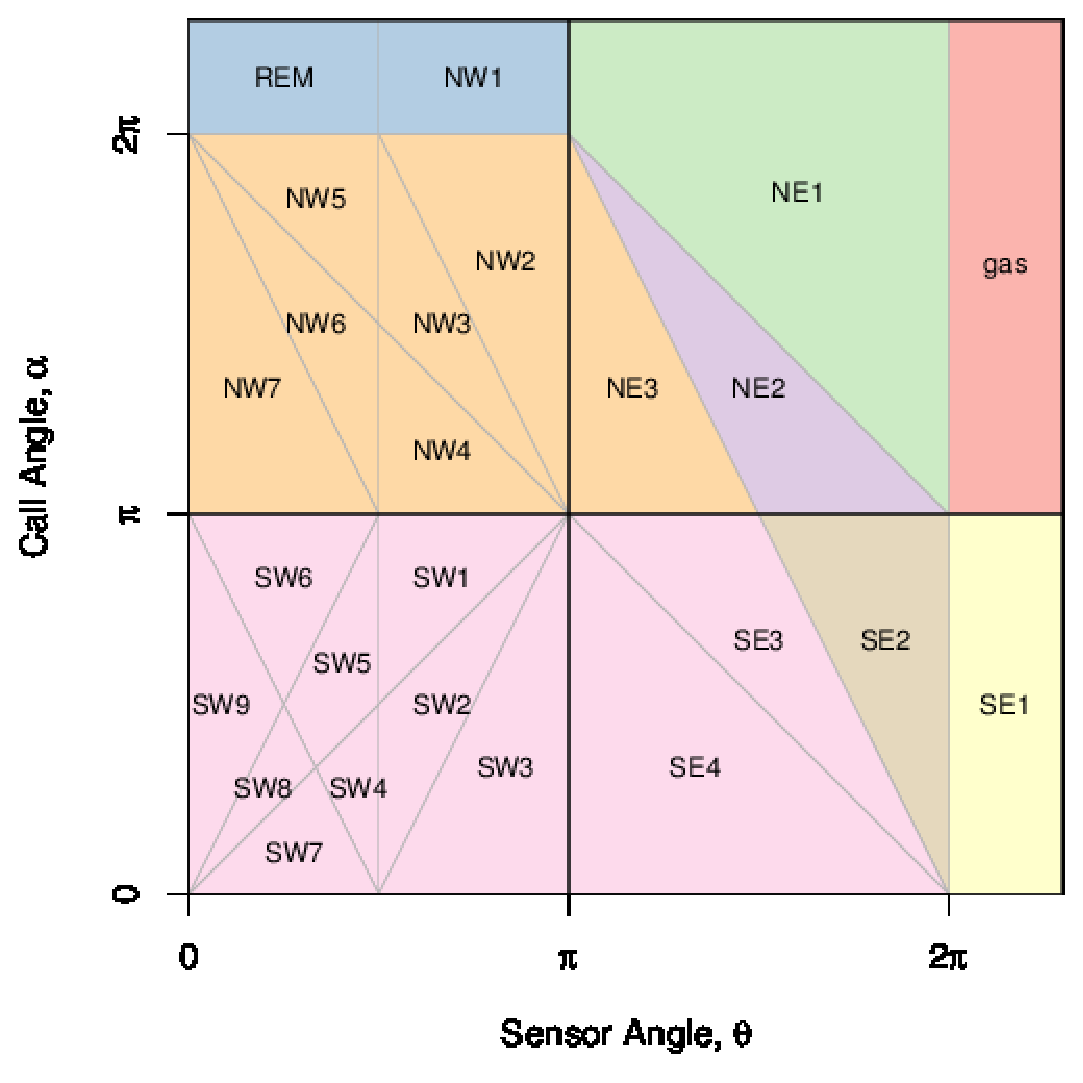
\includegraphics[width=1\textwidth]{imgs/equalRegions.eps}
\caption{The independently derived models for the whole of parameter space. Regions whose solution for $p$ are equal are coloured similarly. Models are numbered by their row, column and then numbered within that cell. The models for $\alpha = 2\pi$ or $theta =  2\pi$ are shown by extending these regions outside of their real boundaries.}
\label{f:regions}
\end{figure}

Figure \ref{f:regions} shows the different regions with the upper right being the gas model as derived above and p141 is the model from \citep{rowcliffe2008estimating}. Parameter space is broadly split into three rows ($ \alpha \le \pi, \pi \le \alpha < 2π\pi$ and $ \alpha = 2\pi$) and four columns ($ \theta \le \pi/2,  \pi/2 \le \theta \le  \pi,  \pi \le \theta < 2\pi$ and $\theta = 2\pi$) which define rectangular regions we will call cells. The equation for $p$ in each region is denoted by three numbers referring to rows, columns and region within that cell. 

For regions with profiles that are more complex than a circle we need to explicitly write functions for the width of the profile for every approach angle. We then use these functions to find the average profile for all approach angles by integrating across all $2\pi$ angles of approach and dividing by $2\pi$. In practice, as the models are all left/right symmetrical we can integrate across $\pi$ angles of approach and divide by $\pi$.

To work through one example that contains both a and s we will examine p321. Following \citep{rowcliffe2008estimating} we use $\gamma_i$ to denote the focal angle which is the angle we integrate over. The subscript $i$ distinguishes different angles. For model p321 we examine $x_1$ with  $x_1 = \pi/2$ being an approach angle directly towards the sensor (see Figure \ref{f:p231schem}).

We can see that, rotating anticlockwise, from $x_1  = \pi/2$ the detection region is $2r$ wide. However, an animal will only be detected if it approaches the detector so that as it enters the detection region the angle between the direction of approach and the direction towards the sensor is less than $\alpha/2$. The width of the profile within which the animal will be detected is therefore $2r\sin(θa/2)$. At $x_1  = \theta/2 + \pi/2 – \alpha/2$ we reach a point where the right hand side of the profile (relative to the approach direction) isn't limited by the call angle but is limited by the detection angle instead. From here the profile width is therefore $r\sin( \alpha/2) + r\cos( x_1  – \theta/2)$. Finally, at $x_1  = 5\pi/2 - \theta/2  - \alpha/2$ an animal can again be detected from the right side of the detector; the approach angle is far enough round to see past the `blind spot' of the sensor. In this region, until $x_1  = 3\pi/2$, the width of the profile is again $2r\sin( \alpha/2)$. We have therefore characterised the profile width for $\pi$ radians of rotation (from directly towards the sensor to directly behind the sensor.) To find the average profile width for any angle of approach, we integrate these functions over their appropriate intervals of $x_1 $ and divide by $\pi$.
\begin{align}
    p321 =&\frac{1}{\pi} \left(\int\limits_{\frac{\pi}{2}}^{\frac{\pi}{2} + \frac{\theta}{2} - \frac{\alpha}{2}}2 r \sin{\left (\frac{\alpha}{2} \right )}\;\mathrm{d}\gamma_{4}+\int\limits_{\frac{\pi}{2} + \frac{\theta}{2} - \frac{\alpha}{2}}^{\frac{5 \pi}{2} - \frac{\theta}{2} - \frac{\alpha}{2}}r \sin{\left (\frac{\alpha}{2} \right )} + r \cos{\left (\gamma_{4} - \frac{\theta}{2} \right )}\;\mathrm{d}\gamma_{4}+\int\limits_{\frac{5 \pi}{2} - \frac{\theta}{2} - \frac{\alpha}{2}}^{\frac{3 \pi}{2}}2 r \sin{\left (\frac{\alpha}{2} \right )}\;\mathrm{d}\gamma_{4}\right)\\
    p321 =& \frac{r}{\pi} \left(\theta \sin{\left (\frac{\alpha}{2} \right )} - \cos{\left (\frac{\alpha}{2} \right )} + \cos{\left (\frac{\alpha}{2} + \theta \right )}\right)
\end{align}
Then, as with the gas model, this term is used to calculate density
\begin{equation}
D = z/vtp321. 
\end{equation}
We can also see what causes this model to be discontinuously different to p322. Examine the profile at $x_1 = 	\theta/2 + \pi/2$ (the profile is perpendicular to the edge of the blind spot.) We see that there is potentially a case where the left side of the profile is $r\sin( \alpha/2)$ while the right side is zero. This profile doesn't exist if we return to the full $2r\sin( \alpha/2)$ profile before $x_1  = \theta/2 + \pi/2$. Therefore we solve $5\pi/2 - \theta/2 - \alpha/2 <  \theta/2 + \pi/2$. We find that this new profile only exists if $ \alpha < 4\pi - 2 \theta$. This inequality defines the line separating p321 and p322.

While specifying the models had to be done by hand, the calculation of the solutions was done using SymPy \citep{sympy} in Python. 

The models are checked for errors with a number of tests. They are checked against each other by checking that adjacent models are equal at the boundary between them. Models that border $ \alpha = 0$ should have $p = 0$ when $ \alpha = 0$ and this is checked for. We checked that all solutions are between 0 and $2r$ and that each integral, divided by the range of angles that it is integrated over is between 0 and $2r$.

To make the application of these models simple, we have included an R script in S1. 

\subsection{Simulation Methods}

The simulated world consists of $56.25km^2$ and is populated with a density of  70 animals per $km^2$ \cite{damuth1981population}, creating a total of 3937 animal per simulation randomly placed at the start of the simulation. 

The animals move with a simple movement model, where the animals moves in discrete time steps and there is assumed to be continuous movement, and, no directional change at the end each step. The simulation lasts for N steps of length,t, during which the animals move with an average constant speed, v. 

The distance travelled in each time step, $\mathnormal{d}$, is a random distance picked from Normal distribution with mean distance, $\mu_d = \mathnormal{v} \times \mathnormal{t}$,  and standard deviation of $\sigma_d = \frac{\mathnormal{v} \times \mathnormal{t}}{10}$. An average speed, $\mathnormal{v} =$40km/day, was chosen as this represents the largest day range of terrestrial animals \cite{carbone2005far}, and represents the upper limit of realistic speeds.
  
The simulation of movement outputs the details of each individual capture events, including the angle of front of the animal to the sensor, from which the number of capture event can be calculated for different call widths. The total number of capture events are summed and the analytical model applied to the results in order to estimate the density in the simulation. From this the difference between the true, and estimated, densities can be used to evaluate the bias in the analytical models. If the analytical models are correct the mean difference between the two values should converge to zero as sample size increases. 

In order to assess the precision of the analytical models for different sampling conditions and animal behaviours, the results of the movement simulation have been subsampled, and rerun with different movement parameters. The total sampling time that the simulation generates, and density population have been subsampled from the original run. Additional simulations have been run to simulate a range of speeds, between 10m/day through to 40km/day to look at full range of terrestrial movement speeds \cite{carbone2005far}. Additional simulations were also run for more complex movement models, such as, correlated random walks, and stationary, or perching, time steps whilst keeping the same longterm average speed. Further simulations were run to identify the sensitivity of the sensor to changes in the radius and width of the detection angle.





\section{Results}

\begin{itemize}
\item The model equations
	\begin{itemize}
	\item Number of different model extensions that have been calculated
	\item Figure with model numbers in which can be used to reference the appendix?
	\end{itemize}
\item Bias is approximately zero for all models as demonstrated by simulation: 
	\begin{itemize}
	\item At a given speed, density, sampling effort, sensor radius, and a given movement strategy
	\end{itemize}
\item The expected number of captures will vary, dependent on the system that is being monitored and how it is monitored. This will affect the precision of the estimated: 
	\begin{itemize}
	\item Animal movement strategy
	\item Speed of movement
	\item Density of the animal
	\item Sampling effort
	\item Radius of the sensor
	\end{itemize}
\end{itemize}


\section{Discussion}
\begin{itemize}
\item Developed a number of models that can be used to estimate density from acoustic and optical sensors 
\item These models are accurate 
\item Implications for best practice:
	\begin{itemize}
	\item Densities of above X converge quickly to a stable mean
	\item Animals which have an average speed of greater then X 
	\item Surveys of at Xhrs of effort produce stable results
	\end{itemize}
\item Aspirational stuff for the future:
	\begin{itemize}
	\item Consider animals moving in groups
	\item Incorporating more realistic movement strategies
	\item Moving detectors
	\item Trigger delays and time expansion
	\end{itemize}
\end{itemize}




\section{Acknowledgements}
Cheers all.


\section{Data Accessibility}






\begin{table}[t]
\centering
\begin{tabular}{lll}
Symbol 	& Description & Units\\\hline
$v$		& Velocity & Metres per second\\
$\theta$	& Angle of detection & Radians \\
$\alpha$	& Animal call/beam width & Radians \\
$r$ 		& Detection distance & Metres\\
$t$			& Time & Seconds\\
$z$			& Number of dections & \\
$D$		& Animal density & Animals m$^{-2}$ \\
$x_i$	& Focal Angle 	& Radians\\
\end{tabular}
\caption{List of symbols used}
\label{t:paras}
\end{table}



\bibliographystyle{mee.bst}	
\bibliography{lucas-moorcroft-etal-refs.bib}	


\end{document}
		
